%%%%%%%%%%%%%%%%%%%%%%%%%%%%%%%%%%%%%%%%%
% "ModernCV" CV and Cover Letter
% LaTeX Template
% Version 1.1 (9/12/12)
%
% This template has been downloaded from:
% http://www.LaTeXTemplates.com
%
% Original author:
% Xavier Danaux (xdanaux@gmail.com)
%
% License:
% CC BY-NC-SA 3.0 (http://creativecommons.org/licenses/by-nc-sa/3.0/)
%
% Important note:
% This template requires the moderncv.cls and .sty files to be in the same 
% directory as this .tex file. These files provide the resume style and themes 
% used for structuring the document.
%
%%%%%%%%%%%%%%%%%%%%%%%%%%%%%%%%%%%%%%%%%

%----------------------------------------------------------------------------------------
%	PACKAGES AND OTHER DOCUMENT CONFIGURATIONS
%----------------------------------------------------------------------------------------
% ModernCV with BibLaTeX-based Multi-section Publications
\documentclass[11pt,letterpaper,sans]{moderncv}

% ModernCV theme
\moderncvstyle{classic}
\moderncvcolor{purple}

% Geometry
\usepackage[scale=0.85]{geometry}


% BibLaTeX setup 
\usepackage[backend=biber,style=ext-verbose,sorting=ydnt]{biblatex}
\usepackage{pdfpages}
\ExecuteBibliographyOptions{doi=true, url=true, isbn=false}

\addbibresource{journal.bib}
\addbibresource{conference.bib}
\addbibresource{corresponding.bib}
\addbibresource{whitepapers.bib}
\addbibresource{talks.bib}
\addbibresource{gradthesis.bib}
\addbibresource{ugradthesis.bib}
\addbibresource{software.bib}
\addbibresource{internal.bib}

% Declare categories
\DeclareBibliographyCategory{journal}
\DeclareBibliographyCategory{conference}
\DeclareBibliographyCategory{corresponding}
\DeclareBibliographyCategory{whitepapers}
\DeclareBibliographyCategory{talks}
\DeclareBibliographyCategory{gradthesis}
\DeclareBibliographyCategory{ugradthesis}
\DeclareBibliographyCategory{software}
\DeclareBibliographyCategory{achievements}

% categorize entries by source file
\AtBeginDocument{%
  \nocite{*} % Load all entries from all .bib files
  %\forcsvlist{\addtocategory{journal}}{bird2025balrog, cannon2025guidelines, drolet2024increased, v15102108, 10.1371/journal.pone.0235303, yiyuan2019epps, ho2018single, cumming2016future}
}

% Font & links
\usepackage{fontawesome5}
\usepackage{marvosym} 
\usepackage{academicons}
%\usepackage[colorlinks]{hyperref}

%----------------------------------------------------------------------------------------
%	NAME AND CONTACT INFORMATION SECTION
%----------------------------------------------------------------------------------------


% Personal Data
%\firstname{David}
%\familyname{Molik}
%\title{Curriculum Vitae}
%\address{University Library}{Kansas State University}
%\mobile{+1 (716) 982-5235, +1 (785) 532-5399}
%\email{molik@ksu.edu} 
%\homepage{http://david.molik.co}{david.molik.co}
%\extrainfo{
%  \faGithub\href{https://github.com/molikd}{ molikd} \quad
%  \faLinkedin\href{https://www.linkedin.com/in/dmolik/}{ dmolik} \quad
%  \aiOrcid\href{https://orcid.org/0000-0003-3192-6538}{ 0000-0003-3192-6538}
%}

%\social[linkedin][www.linkedin.com]{name}
% The first argument is %the url for the clickable link, the second argument is the url displayed in the %template - this allows special characters to be displayed such as the tilde in this %example

%\photo[70pt][0.3pt]{picture} % The first bracket is the picture height, the second is %the thickness of the frame around the picture (0pt for no frame)
%\quote{Not Attention, Patience is all we need.}

%----------------------------------------------------------------------------------------


\newcommand{\cvdoublecolumn}[2]{%
  \cvitem[.75em]{}{%
    \begin{minipage}[t]{\listdoubleitemcolumnwidth}#1\end{minipage}%
    \hfill%
    \begin{minipage}[t]{\listdoubleitemcolumnwidth}#2\end{minipage}%
    }%
}


%\usepackage{multibbl}
\newcommand\Colorhref[3][violet]{\href{#2}{\color{#1}#3}}

\begin{document}

% --- Cover Page ---
\begin{titlepage}
    \raggedright
    \vspace*{1.25in}

    {\color{color1}\LARGE\bfseries Tenure and Promotion Portfolio\par}
    \vspace{0.25in}

    {\color{color1}\rule{\textwidth}{1.5pt}}

    \vspace{0.75in}

    {\Large David Molik, Ph.D.\par}
    \vspace{0.15in}

    {\normalsize Associate Professor\par}
    {\normalsize Department Head, Open Publishing Exchange\par}
    {\normalsize Kansas State University Libraries\par}

    \vspace{0.75in}

    {\normalsize Submitted for Consideration of Tenure\par}

    \vfill

    {\normalsize \today\par}
\end{titlepage}
\newpage

% recomendation form
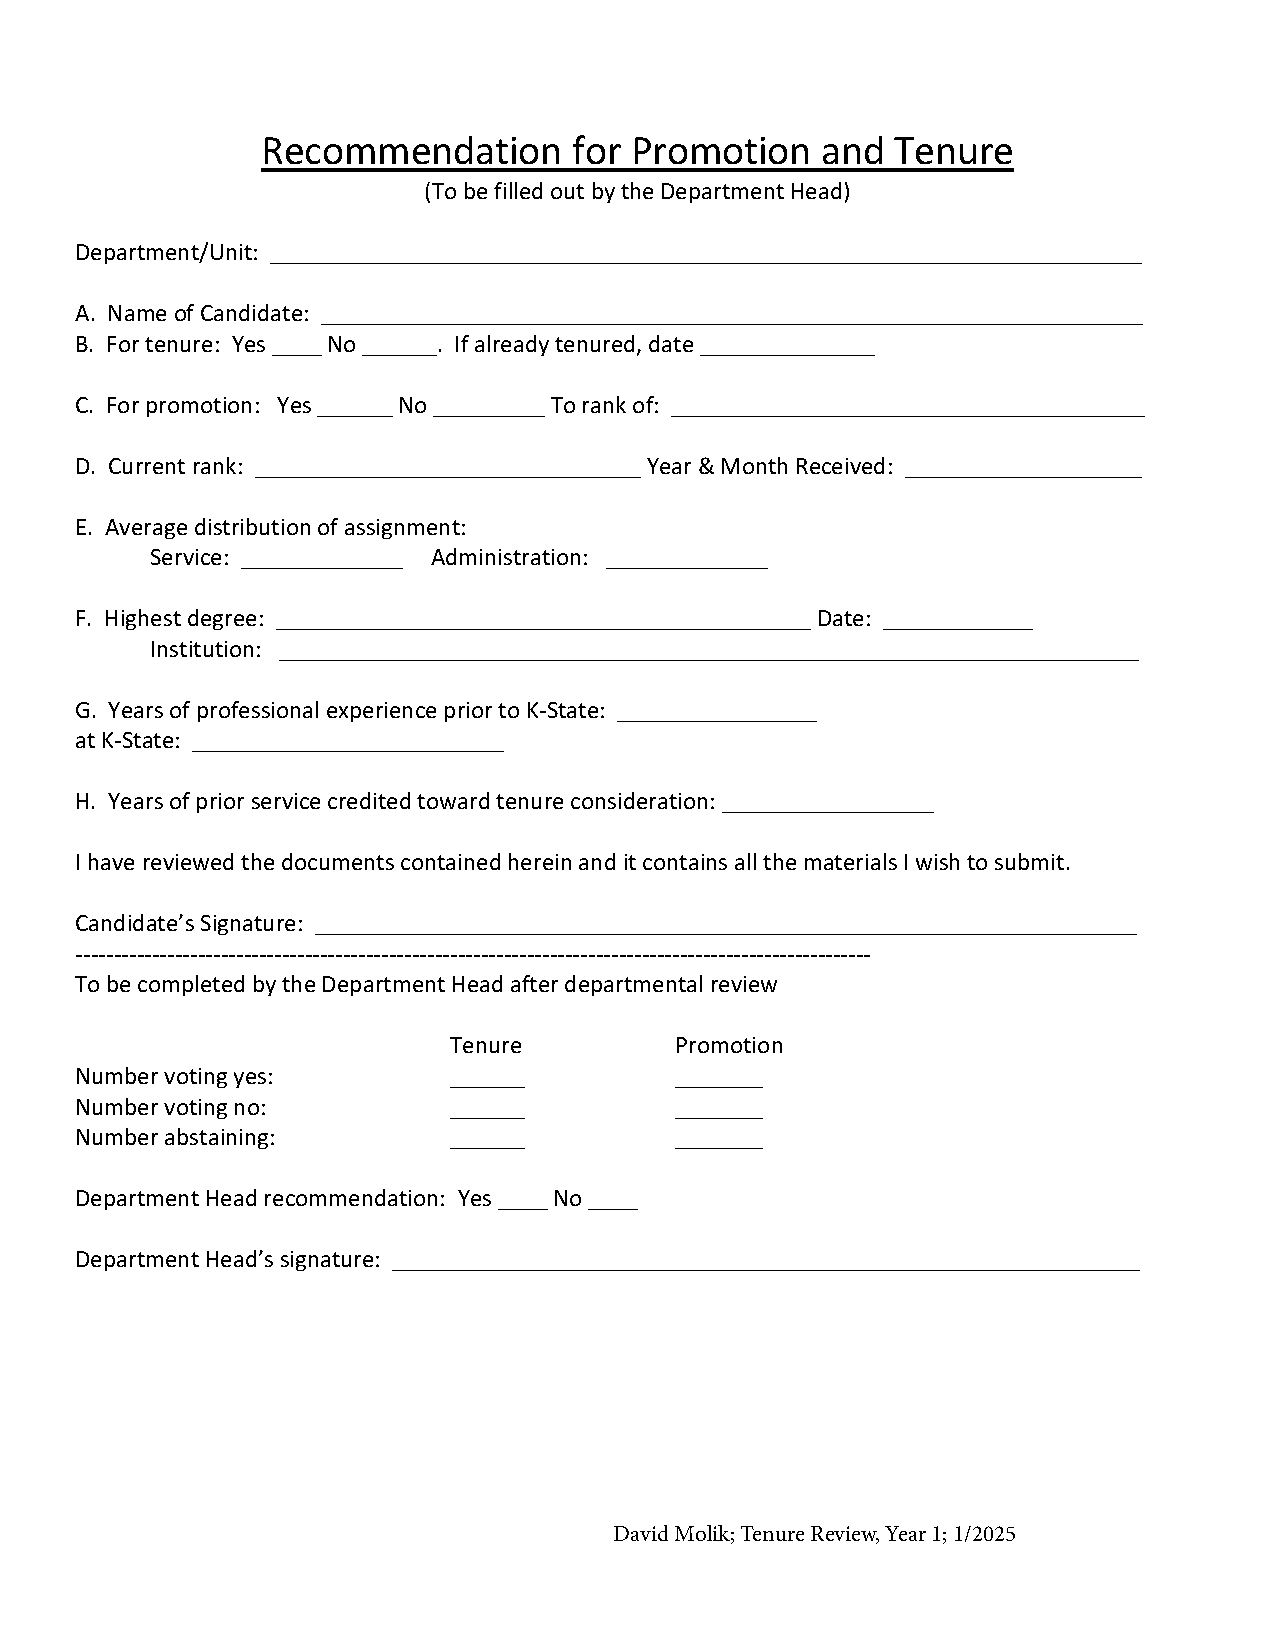
\includepdf[pages=-]{recomendation.pdf}


% --- Employment History ---
\clearpage
\thispagestyle{empty}

\vspace*{0.75in}
{\raggedright

{\color{color1}\Large\bfseries Employment History\par}
\vspace{0.25in}
{\color{color1}\rule{\textwidth}{1pt}}

\vspace{0.6in}

\begin{tabular}{@{}ll@{}}
\textbf{Appointment Date at K-State:} & February 25, 2025 \\
\textbf{Mid-Probation Review Date:} & December 2027 \\
\textbf{Final Tenure Review Date:} & December 2030 \\
\textbf{Annual Status Worksheet:} &
\href{https://staffnet.lib.k-state.edu/display/HR/Annual+Status+Worksheet}
{staffnet.lib.k-state.edu/display/HR/Annual+Status+Worksheet} \\
\end{tabular}

}
\newpage

% Include Achivements
% 2026 narrative draft; source mapping and open items are in planning/2026-draft-status.md.
% Shared presentation remains in shared/preamble.tex.
\firstname{David}
\familyname{Molik}
\title{Statement of Accomplishments -- 2026}
\address{University Library}{Kansas State University}
\portfoliotitle

\section{Research infrastructure through library leadership}
My work connects scholarly communication, computational genomics and research-data stewardship. In 2026, I developed this agenda through leadership of the Open Publishing Exchange (OPE), service as Lead Research Officer for K-State Libraries, faculty mentoring, grant development and research software. My earlier publications and appointments provide the foundation for this work; the activities below emphasize the current year through September 15. The cumulative CV retains prior professional achievements.\evidenceref{L1}

\subsection*{Building people and institutional capacity}
As OPE Department Head, I translated service priorities into student roles with named librarian mentors, technical training and increasing responsibility. I revised position descriptions, coordinated approval and HR posting, and participated in onboarding three students into the departmental communication space. The three postings were confirmed on August 10; the subsequent onboarding is documented separately. I also designed an initial paid training pathway for supervisors to use. These are completed staffing and mentoring actions; student learning and retention remain longer-term outcomes.\evidenceref{L2}

My research leadership included sustained mentoring of Gwen Sibley's William T. Grant letter of inquiry. Across July drafts, I advised on the research gap, methods, evidence-use framing, sponsor fit and biosketch; her replies identify suggestions incorporated into revisions. With Jeff Sheldon, I developed and delivered a Sunderland operating model linking research support, workforce pathways and grant opportunities. I also contributed grant-development resources in a September conversation with Carol Sevin and convened an IUSE planning team. These examples demonstrate how I help colleagues turn ideas into research plans without equating planning with awarded funding.\evidenceref{L3}\evidenceref{L4}

\subsection*{Making research information usable}
In response to the Vice President for Research's request, I contributed publication-indicator analysis and developed HAIL, HAIL-local and related dashboard prototypes. The work connects source reconciliation, caching, provenance and reporting to institutional research questions. Preliminary reports and repository changes establish implementation and review activity. Stakeholder correspondence recognizes progress; validated recurring refreshes and evidence of decisions informed by the reports remain forthcoming.\evidenceref{K1}

I also coordinated research-data and publishing service development, including follow-up resources for the May data-curation workshop and a published Research Weekly explanation of the serials crisis. The latter received favorable feedback relayed by Libraries leadership.\evidenceref{D1}

\subsection*{Research, funding and professional contribution}
I served as PI/project director for Ag-DEx, submitted June 26 with a federal request of \$923,325; it was not funded. I was PI for the \$9 million K-FORGE proposal submitted July 28. I received an ID3A seed-funding commitment of \$13,417, and submitted a \$449,912.20 FFAR application. Each represents a different stage of research development, and the detailed narrative separates awards, submissions and concepts.\evidenceref{G1}

I co-authored the 2026 \textit{Genetics} article \textit{Toward standardization in arthropod and biodiversity genome projects}, contributed to manuscript revision and meeting-report preparation, and advanced computational tools through documented software changes. As an AgBioData co-PI and K-State subcontract PI, I contributed meeting, budget and team coordination. The Mission and Leadership Award recognized my AgBioData service in April.\evidenceref{R1}\evidenceref{R2}\evidenceref{S1}

My institutional service included LFPS Vice Chair responsibilities and recommendations incorporated into revised promotion-and-tenure guidance. Externally, I continued i5k and AgBioData leadership, undertook review assignments and became a guest editor for a launched ecology and evolution special collection. Together, these activities show a coherent contribution to the people, standards and infrastructure that make research accessible and reusable.\evidenceref{N1}\evidenceref{N2}

\newpage

% Include Personal Goals
% 2026 narrative draft; source mapping and open items are in planning/2026-draft-status.md.
% Shared presentation remains in shared/preamble.tex.
% These goals update the 2025 five-year commitments rather than replacing
% them: each entry restates the original commitment, notes progress, and
% gives the updated direction. Measurable targets are retained where still
% applicable and revised where the work has changed.
\firstname{David}
\familyname{Molik}
\title{Five-Year Goals -- 2027--2031}
\address{University Library}{Kansas State University}
\portfoliotitle

\begingroup
\setlength{\parindent}{1.5em}
\setlength{\parskip}{0.45em}
\section{Updated five-year goals}
The 2025 portfolio set nine commitments across directed service,
non-directed service, and research and creative activity. The goals below
carry each commitment forward: what was pledged, what has happened since,
and where it goes next. Targets and dates remain proposals for discussion
with my supervisor, not an approved performance agreement.

\subsection{Directed Service}
\textbf{Strategic plan implementation (2025 pledge: execute the CSP 2025--2030
strategic plan; grow New Prairie Press monographs).} The departmental
landscape document and executive summary (July 2025) now serve as planning
references, and the Center for Scholarly Publishing has become the Open
Publishing Exchange. Through 2027--2031 I will execute the plan's priorities
-- publishing infrastructure, open educational resources, and research-data
services -- and sustain monograph growth, adjusting year-on-year targets as
the revised OATI committee structure takes effect.

\textbf{Research compliance and infrastructure (2025 pledge: a FAIR-aligned
institutional data repository; Library--OVPR liaison on CRIS/RIMS with at
least two joint initiatives).} Coordination with the Office of Research and
Research IT is underway, including repository planning and research-data
management development. Through 2027--2031 I will bring the repository
selection (Figshare, Dataverse, or equivalent) to a decision, complete at
least two Library--OVPR initiatives, and align services with Nelson Memo
compliance needs.

\textbf{Scholarly publishing partnerships (2025 pledge: a Kansas library
publishing initiative of at least five institutions meeting monthly with 20\%
cost reduction; Janeway/Fulcrum engagement; two additional science journals).}
Migration of New Prairie Press toward Fulcrum/Janeway is in progress. Through
2027--2031 I will formalize the Kansas partnership, maintain coalition
engagement, and add science titles where demand and capacity support them,
revising the cost and cadence targets against actual membership.

\subsection{Non-Directed Service}
\textbf{Library-academic collaboration (2025 pledge: at least three grant
submissions as co-investigator; at least two project collaborations outside
the library).} Co-investigator roles on the AgBioData Research Coordination
Network, the DoD xenosurveillance project, and NSF award 2126334, together
with data-publishing and AI-workflow collaborations, meet the substance of
this pledge. Through 2027--2031 I will continue joint proposal development
with faculty at a comparable pace, prioritizing awards over submissions.

\textbf{Library talent (2025 pledge: onboarding support; two workshops per
year).} The OPE student
cohort and Applied Learning Experience pathway now structure onboarding, and
Carpentries and BIP Week instruction continue. Through 2027--2031 I will
mature the onboarding pathway with supervisors, keep training materials
current, and document feedback on role clarity and learning.

\textbf{Professional communities (2025 pledge: AgBioData, BIO-ISAC, and i5k
leadership; yearly conference presence; two scholarly-communication journal
articles).} All three leadership roles continue, with expanded
responsibilities (i5k Training Working Group, AgBioData sustainability work).
Through 2027--2031 I will retain these roles where my expertise is most
useful, attend key conferences yearly, and publish on scholarly-communication
practice.

\subsection{Research, Scholarly and Creative Activity}
\textbf{Scholarly-communication research (2025 pledge: at least one
peer-reviewed article or white paper per year on open publishing
infrastructure, FAIR implementation, and computational methods).} Three
peer-reviewed articles appeared in 2025 with a fourth, on genome reporting
standards, in 2026. Through 2027--2031 I will maintain the yearly pace,
focusing on publishing infrastructure, FAIR implementation, and the methods
behind the tools described below.

\textbf{Cyberbiosecurity publishing (2025 pledge: launch and direct
\textit{Cyberbiosecurity Quarterly}; build the board; seek indexing and
visibility by 2028).} The journal has launched with editorial governance and
peer-review workflows in place. Through 2027--2031 I will grow the editorial
board and submissions and pursue indexing and visibility on the original 2028
horizon.

\textbf{Tools and standards (2025 pledge: GAAN and FHR metadata development
plus at least one software tool; at least two whitepapers).} Open-tool and
metadata-standards work continues through the OPE portfolio and reproducible
research software. Through 2027--2031 I will ship maintained tool releases
tied to methodological questions and co-author whitepapers on preservation,
retention policy, and AI-augmented metadata workflows.

\textbf{Annual review, 2027--2031.} Throughout this period, I will strengthen
my library-science and assessment knowledge and connect it to practice. Before
each annual review, I will update the evidence register, assess progress with
my supervisor and revise goals to reflect responsibilities and available
resources.

\par\endgroup

\newpage

% Include Directed
% 2026 narrative draft; source mapping and open items are in planning/2026-draft-status.md.
% Shared presentation remains in shared/preamble.tex.
\firstname{David}
\familyname{Molik}
\title{Directed Service -- 2026}
\address{University Library}{Kansas State University}
\portfoliotitle

\section{OPE Department Head and Lead Research Officer}
My assigned leadership responsibilities connect open publishing, research-data services and institutional research capacity. The Lead Research Officer MOU describes proposal and partnership development, collaborative funding, project scoping, writing and budgeting. The May 1 administrative correspondence confirms execution of the agreement, and August 5 Strategic Leadership Council minutes corroborate the role and my attendance. This complements my continuing OPE Department Head appointment.\evidenceref{L1}

\subsection*{Supervision, delegation and mentoring}
I developed three student roles spanning data/digital scholarship, publishing/repositories and OER/accessibility. The July--August correspondence records my rationale for early recruitment, meaningful technical work, a primary librarian mentor and increasing responsibility. I revised the descriptions, obtained approval, and sent them to HR. HR confirmed all three Handshake postings and supervisor ownership on August 10. September Teams records document the addition and welcome of three students. I proposed a paid initial open-science training pathway and authorized supervisors to use it; completion and learning outcomes are not yet documented.\evidenceref{L2}

I supported faculty research development through iterative mentoring rather than a single consultation. In July, I reviewed Gwen Sibley's William T. Grant letter of inquiry, focusing on research questions, the distinction between data and research evidence, methods, sponsor alignment and biosketch presentation. Her July 22--23 replies describe incorporating my recommendations, and I circulated Draft 8 on July 24. This provides direct evidence of advice used in revision while preserving her authorship and project ownership.\evidenceref{L3}

I also delegated OPE representation for an Academic Services session and secured access to Carpentries instructor-training opportunities for colleagues. The correspondence establishes coordination and access, not subsequent presentation delivery or certification.\evidenceref{L2}\evidenceref{D1}

\subsection*{Developing research partnerships and services}
Following an August 11 discussion with Jeff Sheldon, I delivered a Sunderland operating-model workbook to Jeff, Tara Coleman and James Wiser on August 12. The accompanying analysis connected ATE/IUSE opportunities to a sustainable research-support program and distinguished routine services from advanced technical and research responsibilities. Jeff's response recognized the write-up. By September 11, we had deferred the ATE application to the following year to strengthen the MATC relationship and other partnerships. The delivered model is the accomplishment; implementation and a funded program remain prospective.\evidenceref{L4}

On September 1, I met with Carol Sevin about grant development and shared USDA/NSF capacity-building resources in the meeting chat. Separately, Carol confirmed incorporating my ORCID suggestion into research guidance on September 2. With melia fritch, Gwen Sibley and Jeff Sheldon, I began developing an IUSE concept examining maker-based learning, STEM self-efficacy and transfer across disciplines. I identified the opportunity, formulated a comparative question, recruited collaborators and shared an example before the September 16 planning meeting. This draft reports preparation, not outcomes of that future meeting.\evidenceref{L4}

For Cassandra Olds's SAS concept, I developed an OPE data-infrastructure scope with an initial technical leadership role for me and a transition to Gwen Sibley's operational RDM leadership. The proposed five-year OPE component totals \$448,798; this is neither the full project budget nor an award. I also developed proposed open-research/publishing services for the OAK-AI Hub discussion. These activities demonstrate service scoping and partnership development, with sponsor and implementation outcomes still separate.\evidenceref{G1}

\subsection*{Research-publication reporting}
The June 1 OVPR request asked Libraries to help assess publication indicators and support NextGen reporting. My response addressed citation windows, affiliations, source quality, open-access categories and research outputs beyond articles. I coordinated Libraries participation and developed complementary infrastructure and reporting approaches. HAIL separates normalized, provenance-aware collection from presentation; HAIL-local provides a cached reporting route; Prairie Observatory explored lightweight repository/dashboard views. These are related efforts serving one institutional need, not three independent impact claims.\evidenceref{K1}

August--September correspondence and reports establish preliminary output generation and review. Hans Coetzee praised development progress on August 27, and Lowell Scott provided positive visual feedback in September. Report versions differ, however, and an August 31 fetching log was followed by a failure notice for that job. I therefore report prototype development, design decisions and preliminary delivery, while reserving claims about reliable full refreshes, final institutional metrics and decision use for validated evidence. Namratha Kommineni's Power BI prototype is a collaborator's contribution, not my sole work.\evidenceref{K1}

\subsection*{Publishing, data stewardship and outreach}
I coordinated service-development discussions following the reported K-REx DSpace 9.3 upgrade, addressing ORCID, OpenAIRE, Crossref, preservation and research-reporting interfaces. This is coordination and planning evidence, not a claim that I personally performed the upgrade or completed every integration. My June Research Weekly article, ``What is the Serials Crisis?'', translated publishing conditions for the campus community; leadership correspondence confirms publication and favorable qualitative response. I provided participants with follow-up research-data and publishing resources after the May 29 workshop.\evidenceref{D1}

The achievements record also documents Textbook 2.0 receipts of \$1,920 against \$385 in 2025, and a consultation involving approximately 250 TB of research data. These figures describe the reported fundraising comparison and consultation scale; they do not establish student savings or data deposited. An identified Green OA route for two chapters similarly remains a possible cost-avoidance opportunity, not realized savings.\evidenceref{D2}

\newpage

% Include Non-Directed
% 2026 narrative draft; source mapping and open items are in planning/2026-draft-status.md.
% Shared presentation remains in shared/preamble.tex.
\firstname{David}
\familyname{Molik}
\title{Non-Directed Service -- 2026}
\address{University Library}{Kansas State University}
\portfoliotitle

\section{Institutional and professional service}
My service beyond assigned departmental responsibilities focuses on faculty governance and the communities that sustain interoperable research data. Overlap with assigned work is identified for supervisor review; grant administration and OPE operations are described in their primary sections rather than counted again here.

\subsection*{Libraries governance}
I serve as LFPS Vice Chair, a role identified in my June correspondence and subsequently confirmed in the evidence review. In the June promotion-and-tenure consultation, I recommended clarifying external-reviewer definitions and the treatment of internal evaluative statements. Margaret Mohr-Schroeder's June 23 response explicitly confirms changes to the revised guidance. In July, I advised Conner Dillard on recruitment, representation and wording for the tenure-and-promotion ad hoc committee's proposed charge. These are concrete governance contributions, without implying that the revised procedures had taken effect.\evidenceref{N1}

\subsection*{Research-data communities}
I continued serving on the i5k Executive Committee, chairing its Training Working Group and participating in the Standards Working Group. The 2026 records include training/community presentations and executive participation. I also continued AgBioData Steering Committee and working-group service and received its Mission and Leadership Award in April. My September 11 appointment as Sustainability Working Group co-chair and acceptance as a future PAG workshop co-organizer establish new leadership responsibilities; the future workshop is not counted as delivered.\evidenceref{N2}

These roles connect agricultural and biodiversity research communities with Libraries expertise in publishing, persistent identifiers and data stewardship. AgBioData's annual meeting and funded coordination are described under RSCAD; they are not additional independent outputs merely because they also support professional service.\evidenceref{R2}

\subsection*{Editorial and peer-review service}
I became a guest editor for \textit{Cyberinfrastructure and Data Management in Ecology and Evolution}, a special collection in \textit{Ecology and Evolution}. The August 14 launch correspondence and public call establish the collection and editorial role, with submissions invited through August 31, 2027. This is an active editorial responsibility, not a completed issue.\evidenceref{N2}

The achievements record identifies four article-review and six meta-review assignments for the First International Workshop on Cyberbiosecurity. I report these as ten assignments, not necessarily ten distinct manuscripts. My PCI Genomics recommendation is also editorial/review service and is not classified as an authored research article. The cumulative CV retains my continuing BIO-ISAC advisory and founding editorial roles.\evidenceref{N2}

\newpage

% Include Research and Creative
% 2026 narrative draft; source mapping and open items are in planning/2026-draft-status.md.
% Shared presentation remains in shared/preamble.tex.
\firstname{David}
\familyname{Molik}
\title{Research, Scholarly and Creative Activity -- 2026}
\address{University Library}{Kansas State University}
\portfoliotitle

\section{A research agenda for reusable scientific information}
My research links computational genomics with the standards, software and publishing practices needed to make scientific information reusable. This is directly relevant to Libraries research support: questions about provenance, interoperability and sustainable access become both methodological problems and service-design requirements.

\subsection*{Publications and manuscripts}
I co-authored \textit{Toward standardization in arthropod and biodiversity genome projects} (\textit{Genetics}, 2026), extending my collaborative work on genomic reporting and interoperability. The article is a published output. In contrast, \textit{The Future is FAIR: A Community Framework for Enhanced Data Management and Data Sharing} is documented through a revised manuscript and reviewer response, and \textit{AgBioData Annual Meeting 2026: Toward Sustainable Agricultural Genomics Infrastructure} through a manuscript-preparation file. I report the latter two as work in progress, not accepted publications.\evidenceref{R1}

The cumulative CV records the earlier \textit{AgBioDatabase Finder}, BALROG-MON and genome-nomenclature articles. They provide context rather than new 2026 publication counts. In particular, BALROG-MON's February 19, 2025 publication precedes the February 25 K-State appointment recorded in the portfolio.

\subsection*{Awards, submissions and project development}
The following activity demonstrates development of a research program; requested budgets are not awarded funding.\evidenceref{G1}
\begin{itemize}
\item \textbf{ID3A seed funding, awarded:} a March 11 letter commits \$13,417 for ``Development of AI-ready digital ag research platform,'' starting March 12. Correspondence documents spending coordination; final expenditure reconciliation and reporting remain to be retained.
\item \textbf{Ag-DEx, submitted and not funded:} as PI/project director, I coordinated proposal components, collaboration materials, personnel and successive narrative drafts. The final package names Gwen Sibley as co-PD/co-PI. USDA received the application June 26 (2026-07893), requesting \$923,325 for January 2027--December 2029; the not-funded status was recorded August 27. Later response work addresses possible revisions rather than a completed resubmission.
\item \textbf{K-FORGE, submitted:} I served as PI with Nicholas Eggleston and Jeffrey Sheldon as co-PIs for ``Category II: K-FORGE: A Federated Open Research Gateway for Executable, Reproducible, and AI-Enabled Science.'' NSF's notification records July 28 submission, proposal 2638522. The request is \$9 million over 36 months, with a proposed February 2027 start. The proposal describes my intended leadership, coordination and governance responsibilities; no funding decision is established by the retained evidence.
\item \textbf{FFAR, submitted:} ``Unlocking Agricultural Research Data for Better Farming Decisions'' was submitted April 29, requesting \$449,912.20 for 2027--2029. This is a full application, not only institutional clearance; an award is not established.
\item \textbf{FAIROS, submitted then withdrawn:} NSF proposal 2624126, ``Disciplinary Improvements: AI-Ready Genome Notes: An Open Science Infrastructure for Rapid, Structured Genomic Reporting,'' was submitted April 8 and withdrawn June 8. Withdrawal is distinct from a sponsor decline.
\end{itemize}
SAS, Sunderland ATE/IUSE and OAK-AI development are described under Directed Service as partnership and project-scoping contributions. They are not added to the submitted-proposal or award totals.

\subsection*{Community research coordination and instruction}
As AgBioData co-PI and K-State subcontract PI, I contributed to the 2026 hybrid community meeting through budget, team and meeting coordination. The annual-report preview identifies these responsibilities but does not prove submission of that report. I also contributed to follow-up and meeting-report development. Survey calculations remain for a later review; I do not convert an AI-generated debrief into verified participation or learning metrics.\evidenceref{R2}

The May data-curation workshop records and follow-up correspondence document educational engagement and participant support. The schedule identifies May 1 and May 29 events; it does not establish my individual instructional hours or attendance totals. Earlier reported 2026 scholarly presentations remain in the evidence inventory for program/material reconciliation rather than being assigned uncertain conference editions here.\evidenceref{D1}

\subsection*{Research software and reproducibility}
I directed and reviewed software development extending my computational research. Barcode Simulator's August--September changes add distance-matrix and graph outputs, compressed/FASTQ output, reproducible run metadata and storage checks. These are software-maintenance and reproducibility contributions, not new biological findings; synthetic FASTQ qualities do not constitute an instrument-error model. PathwayByWire's August work includes pathway-completeness analysis, KEGG exports and an OpenAPI interface. Its conservation/evidence calculations should not be interpreted as measured expression or activity.\evidenceref{S1}

For HAIL, merged September changes implement three-valued bibliometric observations, quality signals, harvest coverage, Janeway enrichment and normalization replay. These are stronger evidence than architectural plans, but remain distinct from a validated production harvest. The institutional purpose and preliminary reporting outputs are described under Directed Service. Repository history includes collaborators and AI-assisted development; my contribution is research direction, design decisions and review, without claiming sole manual authorship of all code.\evidenceref{S1}\evidenceref{K1}

\newpage

% Position Descripton
% recomendation form
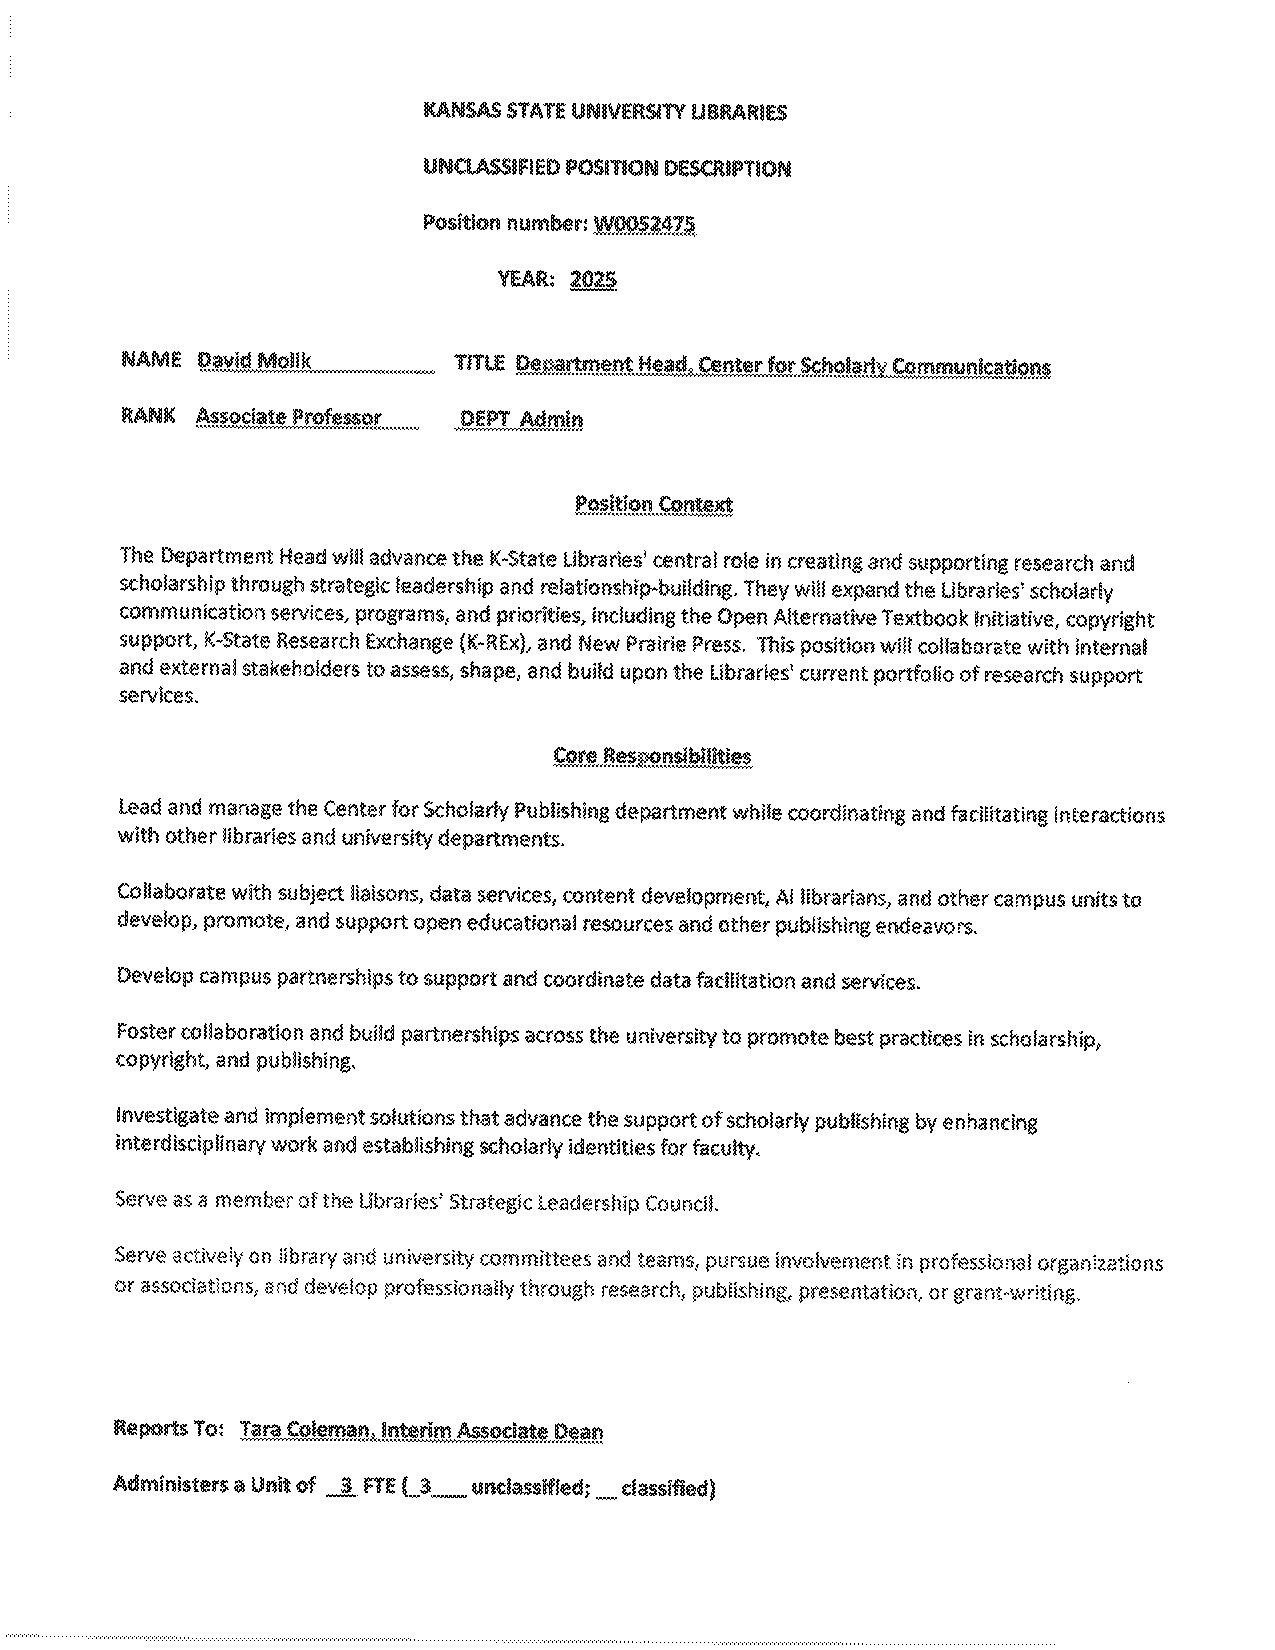
\includepdf[pages=-]{pd.pdf}

% Evaluation
% recomendation form
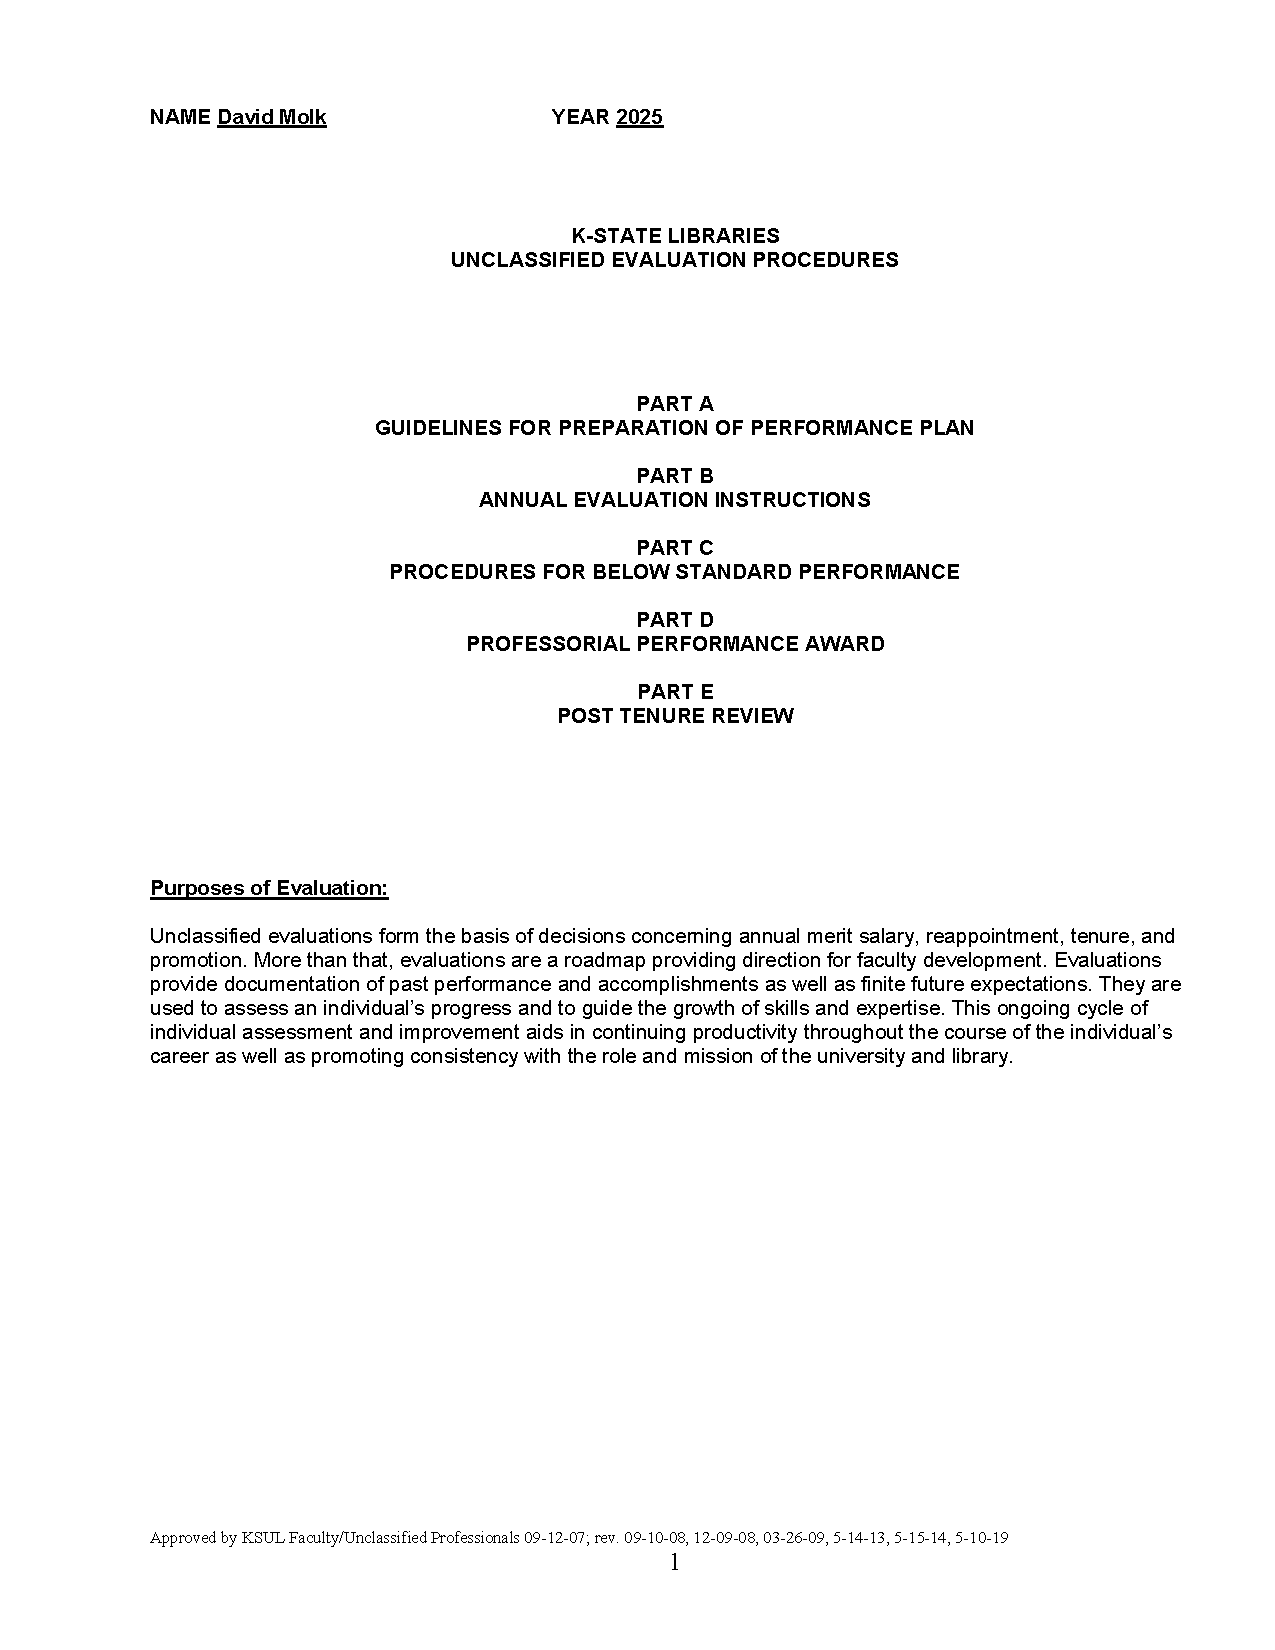
\includepdf[pages=-]{evaluation.pdf}

% Include CV


%----------------------------------------------------------------------------------------
%	NAME AND CONTACT INFORMATION SECTION
%----------------------------------------------------------------------------------------
\defbibheading{none}{}

% Personal Data
\firstname{David}
\familyname{Molik}
\title{Curriculum Vitae}
\address{University Library}{Kansas State University}
\mobile{+1 (716) 982-5235, +1 (785) 532-5399}
\email{molik@ksu.edu} 
\homepage{http://david.molik.co}{david.molik.co}
\extrainfo{
  \faGithub\href{https://github.com/molikd}{ molikd} \quad
  \faLinkedin\href{https://www.linkedin.com/in/dmolik/}{ dmolik} \quad
  \aiOrcid\href{https://orcid.org/0000-0003-3192-6538}{ 0000-0003-3192-6538}
}

%\social[linkedin][www.linkedin.com]{name}
% The first argument is %the url for the clickable link, the second argument is the url displayed in the %template - this allows special characters to be displayed such as the tilde in this %example

%\photo[70pt][0.3pt]{picture} % The first bracket is the picture height, the second is %the thickness of the frame around the picture (0pt for no frame)
%\quote{Not Attention, Patience is all we need.}

%----------------------------------------------------------------------------------------





% \newcommand{\cvreference}[7]{%
%     \textbf{#1}\newline% Name
%     \ifthenelse{\equal{#2}{}}{}{\addresssymbol~#2\newline}%
%     \ifthenelse{\equal{#3}{}}{}{#3\newline}%
%     \ifthenelse{\equal{#4}{}}{}{#4\newline}%
%     \ifthenelse{\equal{#5}{}}{}{#5\newline}%
%     \ifthenelse{\equal{#6}{}}{}{\emailsymbol~\texttt{#6}\newline}%
%     \ifthenelse{\equal{#7}{}}{}{\phonesymbol~#7}}





\portfoliotitle % Repeatable section header (see main.tex)


%----------------------------------------------------------------------------------------
%	WORK EXPERIENCE SECTION
%----------------------------------------------------------------------------------------

\section{Experience}

\subsection{Kansas State University}
\cventry{Feb 2025 -- Present}
  {Department Head, \Colorhref{https://lib.k-state.edu/services-support/scholarly-communication/}{Center for Scholarly Publishing}; Associate Professor}
  {\Colorhref{https://lib.k-state.edu/}{Kansas State University Libraries}}
  {Manhattan, KS}{}%
  {
Provides strategic and operational leadership for the University Libraries’ scholarly communication, open access, and research data programs. Oversees library publishing and repository infrastructure, ensuring sustainable stewardship, metadata interoperability, persistent identifiers, and FAIR data practices. Leads and supports faculty and library staff in advancing digital scholarship, open educational resources, and open science as core library services.
  }

\subsection{United States Department of Agriculture}
\cventry{Mar 2023 -- Feb 2025}
  {Computational Biologist, \Colorhref{https://www.ars.usda.gov/plains-area/mhk/cgahr/abadru/}{Arthropod-borne Animal Disease Research Unit}}
  {USDA ARS}
  {Manhattan, KS}{}%
  {
  Led informatics and data engineering efforts to support genomic surveillance and bioinformatics pipelines for vector-borne disease research. Designed scalable computational workflows for pathogen detection and synthetic gene identification. Coordinated integration of HPC and cloud systems for cross-laboratory data sharing and analysis.
  }

\cventry{Jun 2021 -- Mar 2023}
  {Research Biologist / Postdoctoral Researcher, \Colorhref{https://www.ars.usda.gov/pacific-west-area/hilo-hi/tropical-pest-genetics-and-molecular-biology-research/}{Tropical Pest Genetics and Molecular Biology Research Unit}}
  {USDA ARS}
  {Hilo, HI}{}%
  {
  Conducted bioinformatics and computational genomics research on insect vector populations, focusing on transposable elements and synthetic gene detection. Developed and maintained high-performance analysis pipelines and genomic databases. 
  \textbf{Advisor:} \Colorhref{https://www.ars.usda.gov/pacific-west-area/hilo-hi/daniel-k-inouye-us-pacific-basin-agricultural-research-center/tropical-pest-genetics-and-molecular-biology-research-unit/people/scott-geib/}{Dr. Scott Geib}
  }

%\subsection{Kansas State University}
%\cventry{Feb 2025 -- Present}
%  {Department Head, \Colorhref{https://lib.k-state.edu/https://lib.k-state.edu/services-support/scholarly-communication/}{Center for Scholarly Publishing}; Associate Professor}
%  {\Colorhref{https://lib.k-state.edu/}{Kansas State University Libraries}}
%  {Manhattan, KS}{}%
%  {}
%
%\subsection{United States Department of Agriculture}
%\cventry{Mar 2023 -- Feb 2025}
%  {Computational Biologist, \Colorhref{https://www.ars.usda.gov/plains-area/mhk/cgahr/abadru/}{Arthropod-borne Animal Disease Research Unit}}
%  {USDA ARS}
%  {Manhattan, KS}{}{}
%\cventry{Jun 2021 -- Mar 2023}
%  {Research Biologist / Postdoctoral Researcher, \Colorhref{https://www.ars.usda.gov/pacific-west-area/hilo-hi/tropical-pest-genetics-and-molecular-biology-research/}{Tropical Pest Genetics and Molecular Biology Research Unit}}
%  {USDA ARS}
%  {Hilo, HI}{}%
%  {\textbf{Advisor:} \Colorhref{https://www.ars.usda.gov/pacific-west-area/hilo-hi/daniel-k-inouye-us-pacific-basin-agricultural-research-center/tropical-pest-genetics-and-molecular-biology-research-unit/people/%scott-geib/}{Dr. Scott Geib}}


\subsection{University of Notre Dame, Ph.D. Appointments}
\cventry{Jan 2020 -- Jun 2021}
  {Graduate Scholar, \Colorhref{https://library.nd.edu/services/navari-digital-scholarship/}{Navari Family Center for Digital Scholarship}}
  {University of Notre Dame}
  {Notre Dame, IN}{}{}
\cventry{May 2019 -- Aug 2019}
  {Graduate Research Assistant, \Colorhref{https://www.goodsonlab.org/}{Goodson Lab}}
  {University of Notre Dame}
  {Notre Dame, IN}{}{}
\cventry{May 2018 -- Aug 2018}
  {Graduate Research Assistant, \Colorhref{https://research.nd.edu/cores-and-resources/genomics-and-bioinformatics-core/}{Genomics and Bioinformatics Core Facility}}
  {University of Notre Dame}
  {Notre Dame, IN}{}{}
\cventry{Aug 2016 -- Dec 2017}
  {Graduate Research Assistant, \Colorhref{https://biology.nd.edu/people/scott-emrich/}{Emrich Lab}}
  {University of Notre Dame}
  {Notre Dame, IN}{}{}

\subsection{Pre-Ph.D. Industry Positions}
\cventry{Dec 2014 -- Aug 2016}
  {Scientific Informatics Developer}
  {\Colorhref{https://www.cshl.edu/}{Cold Spring Harbor Laboratory}}
  {Cold Spring Harbor, NY}{}{}
\cventry{Jul 2013 -- Nov 2014}
  {Software Engineer; Network Operations Center Manager}
  {\Colorhref{https://www.synacor.com/}{Synacor}}
  {Buffalo, NY}{}{}

\subsection{Undergraduate Research and Internships}
\cventry{Aug 2012 -- Jan 2013}
  {Undergraduate Researcher, \Colorhref{https://tw.rpi.edu}{Tetherless World Constellation}}
  {Rensselaer Polytechnic Institute}
  {Troy, NY}{}{}
\cventry{May 2012 -- Aug 2012}
  {NSF REU, \Colorhref{https://engineering.buffalo.edu/computer-science-engineering/people/faculty/kenneth-corso.html}{Corso Lab}}
  {SUNY at Buffalo}
  {Buffalo, NY}{}{}
\cventry{May 2010 -- Aug 2010}
  {Intern, \Colorhref{https://tw.rpi.edu}{Tetherless World Constellation}}
  {Rensselaer Polytechnic Institute}
  {Troy, NY}{}{}

%----------------------------------------------------------------------------------------
%	EDUCATION SECTION
%----------------------------------------------------------------------------------------

\section{Education}

\subsection{University of Notre Dame: Ph.D.}
\cventry{Aug 2016 -- May 2021}{Ph.D. in Integrated Biomedical Sciences}{University of Notre Dame}{Notre Dame, IN}{Concentration in Computational Biology}{Dissertation:\printbibliography[keyword={gradthesis},heading=none]}
\cvitem{Advisor:}{\textit{Prof. Michael E. Pfrender}, \textit{Department of Biological Sciences}, Lab Website: \Colorhref{https://pfrenderlab.nd.edu}{https://pfrenderlab.nd.edu}}


\subsection{Rensselaer Polytechnic Institute: B.S.}
\cventry{Aug 2009 -- Dec 2012}{B.S. in Information Technology and Web Science}{Rensselaer Polytechnic Institute}{Troy, NY}{Concentration in Communications}{Thesis:\printbibliography[keyword={ugradthesis},heading=none]}
\cvitem{Advisor:}{\textit{Prof. Deborah L. McGuinness}, \textit{Cognitive and Web Sciences}, Lab Website: \Colorhref{https://tw.rpi.edu/person/Deborah_L_McGuinness}{https://tw.rpi.edu/person/Deborah\_L\_McGuinness}}


%----------------------------------------------------------------------------------------
%	PUBLICATION SECTION
%----------------------------------------------------------------------------------------
% Publications

\section{Publications}
%\subsection{Corresponding Author Articles}
\cvitem{\textbf{Corresponding Author Articles}}{\printbibliography[keyword={corresponding},heading=none]}
%\subsection{Journal Articles}
\cvitem{\textbf{Collaborative Articles}}{\printbibliography[keyword={journal},heading=none]}
%\subsection{Conference Proceedings}
\cvitem{\textbf{Conference Proceedings}}{\printbibliography[keyword={conference},heading=none]}
%\subsection{Chapters and Whitepapers}
\cvitem{\textbf{Chapters and Whitepapers}}{\printbibliography[keyword={chapters},heading=none]}

%----------------------------------------------------------------------------------------
%	Talks
%----------------------------------------------------------------------------------------

\section{Talks}
\printbibliography[keyword={talks},heading=none]


%----------------------------------------------------------------------------------------
%	Funding
%----------------------------------------------------------------------------------------


\section{Grants \& Funding}

\subsection{Research Awards}
\cvitem{2024}{\textbf{K-State Libraries Inaugural Internal Grant} — Spahr, K., McCowen, R., Jackson, C., Otto, R., Sibley, G., Berney, E., Turvey-Welch, M., Misilo, T., Andresen, D., Molik, D.  
\newline \emph{Empowering Data Literacy: Building a Carpentries Community at K-State.}}
\cvitem{2024}{\textbf{Co-PI}, DoD Global Emerging Infections Surveillance Grant – \textit{“Using house flies as xenosurveillance tools to monitor existing, emerging and cryptic microbial threats to US military”} \hfill \textbf{\$150,000}}
\cvitem{2021}{\textbf{Oracle for Research Cloud Award} – Scientific cloud application development \hfill \textbf{\$90,000 in Oracle Cloud Credits}}
\cvitem{2016--2018}{\textbf{AWS Cloud Credits for Research} – Alternative bioinformatics platforms and enrichment pipelines \hfill \textbf{Total: \$60,000}}
\cvitem{2016}{\quad-- Individual Research Cloud Credit \hfill \textbf{\$10,000}}
\cvitem{2017}{\quad-- Co-Investigator Cloud Credit \hfill \textbf{\$30,000}}
\cvitem{2018}{\quad-- Metagenomic Enrichment Pipeline Development \hfill \textbf{\$20,000}}

\subsection{Travel Funding}
\cvitem{2020}{\textbf{University of Notre Dame Zahm Research Travel Grant} – CSHL Biological Data Science}
\cvitem{2019}{\textbf{Notre Dame Zahm Research Travel Grant} – CSHL Genome Informatics \hfill \textbf{\$1,176.43}}
\cvitem{2019}{\textbf{Graduate Student Union Conference Presentation Grant (GSU CPG)} – Entomology 2019}
\cvitem{2018}{\textbf{Graduate School Professional Development Award (Notebaert)} – IEEE BIBM 2018 \hfill \textbf{\$1,000}}
\cvitem{2017}{\textbf{GSU Conference Presentation Grant} – CSHL Genome Informatics 2017}
\cvitem{2017}{\textbf{REACT Program Grant (Rapid Exposure to Advanced Computational Training)} – Computational short course attendance \hfill \textbf{\$1,500}}


%----------------------------------------------------------------------------------------
%    Professional activities SECTION
%----------------------------------------------------------------------------------------

\section{Professional Activities}

\cventry{2023 -- present}{Member, \href{https://i5k.github.io/}{i5k Initiative}}{}{}{}{
  \begin{itemize}
    \item Executive Committee Member, 2025 -- present
    \item Chair, Training Working Group, 2025 -- present
    \item Standards Working Group Member, 2023 -- present
  \end{itemize}
}

\cventry{2023 -- present}{Member, \href{https://www.agbiodata.org/}{AgBioData}}{}{Pullman, WA}{}{
  \begin{itemize}
    \item 2024 Data FAIRification Award
    \item \href{https://www.agbiodata.org/steering-committee-members}{Steering Committee}, 2025 -- present
    \item FAIR Scientific Literature Working Group, 2023 -- present
    \item Genome Assembly and Annotation Nomenclature WG, 2023 -- 2025
  \end{itemize}
}

\cventry{2025 -- present}{Board Member, \href{https://www.isac.bio/}{BIO-ISAC (Bioeconomy Information Sharing and Analysis Center)}}{Advisory Board}{Brooklyn, NY, USA}{}{
  \begin{itemize}
    \item Invited position on Advisory Board
  \end{itemize}
}

\cventry{2025 -- present}{Editorial Board Member, \href{https://newprairiepress.org/cyberbiosecurity/}{\textit{Cyberbiosecurity Quarterly}}}{New Prairie Press}{Manhattan, KS, USA}{}{
  \begin{itemize}
    \item Founding Editor
  \end{itemize}
}


%----------------------------------------------------------------------------------------
%	Teaching  SECTION
%----------------------------------------------------------------------------------------

\section{Teaching}
\subsection{Courses}
\cvitem{Fall 2020}{Instructor, BIOS 60132: \textit{Introduction to Computational Genomics}, University of Notre Dame (3 credit graduate course).}
\subsection{Workshops}
\cvitem{2025}{Certified instructor, Carpentries (bioinformatics workshops) for Kansas State University – delivered summer incoming life sciences workshop.}
\cvitem{2023 -- 2024}{Certified instructor, Carpentries (bioinformatics workshops) for USDA ARS – delivered three in 2023 and one in 2024.}
\cvitem{Summer 2020,2021}{Led “Bioinformatics Introductory Program Week” (BIP Week), Notre Dame Center for Digital Scholarship – 4-day bootcamp for incoming life-sciences graduate students.}
\cvitem{Spring 2020}{Taught Data Carpentries Genomics curriculum (in-person \& online) for Center for Digital Scholarship, University of Notre Dame.}
\cvitem{Spring 2019}{Lecture TA, BIOS 10172: \textit{Biology II: Molecules to Ecosystems}, Instructor: Prof. Joseph O’Tousa, University of Notre Dame.}
\cvitem{Fall 2018}{Lab TA, BIOS 31312: \textit{General Ecology Laboratory}, Instructor: Prof. Dominic Chaloner, University of Notre Dame.}
\cvitem{Spring 2018}{Lab TA, BIOS 21202: \textit{General Biology B Laboratory}, Instructor: Prof. Dominic Chaloner, University of Notre Dame.}

%----------------------------------------------------------------------------------------
%	Other Achievements SECTION
%----------------------------------------------------------------------------------------


\section{Other Achievements}

\cvitem{2021 -- 2022}{\textbf{Founder, \href{https://nvib.io}{nvib.io}} – Launched a limited liability company through the University of Notre Dame IDEA Center to support technology transfer of ‘met’, a thesis-derived data analysis platform.}

\cvitem{2006}{\textbf{Eagle Scout}, Boy Scouts of America – Achieved the highest rank in scouting.}






\end{document}